\documentclass[12pt, letterpaper]{article}
\usepackage[utf8]{inputenc}
 \usepackage[letterpaper, margin=1in]{geometry}
 \usepackage{amssymb}
\usepackage{amsmath}
 \usepackage{enumitem}
\usepackage {listings}
\usepackage{pgfplots}
\usepgfplotslibrary{external}
\usepackage{graphicx}

\title{CS425 Project 2 (Report)\\Dimensionality Reduction and Clustering}
\author{Ksenia Burova}
\date{October \(22^{nd}\), 2017}

\begin{document}
\maketitle

\noindent {\bf Abstract:} In machine learning, dimension reduction is used to simplify a problem without losing any significant data. There can be many experiments done for a large number of features, and it can be way too hard too analyze results when have many dimensions. Simpler model are also more robust on smaller datasets. Clustering is also important when there can be several groups of data in one large data set. Finding those sets may help analyze data as well. In this project, we were given a data file with all the countries in the world and death numbers per 1000 children before 5 years old for 216 years (1800 - 2015). In a first part of the assignment, we had to complete Principal Component Analysis for data visualization. We had to build several plots to find out how many singular values to choose, and looked at results when first two principal components are used.
In a second part of the project, we had to built k-mean clustering algorithm to be used on data from part one, which in my mind was helpful in analyzing which countries have similar results.\\

\begin{enumerate}[label=\Roman*.]

	{\bf \item Tools.}\\
	
	I've used {\bf python} programming language, {\bf numpy} and  {\bf stats} libraries for arithmetic, and {\bf matplotlib} library to built plots for this project.\\
	
	{\bf \item Project Data.} \\
	
	There were two file formats given for this project, .xlms and .csv. I decided to go with .csv for easier parsing. There were many countries in data that were missing all or some values for yearly death rates. My choice for this experiment was to exclude that data because country yearly death rate estimation is not a thing that can be based on other countries in my mind. For that we would have to know how similar countries are in culture, life style, politics, economics,  existence  years and etc. We don't have that much data. I tried to build a 3D plot of data to see if there some things we can observe immediately. \\
	In plot below, countries are labeled 1 - 180 as there are 180 countries in alphabetical order in data file excluding the ones with missing values. As we can clearly see, pretty much for all countries yearly death rate decreases with time. For some countries rates are higher, for some much lower. \\
	
	\begin{center}
		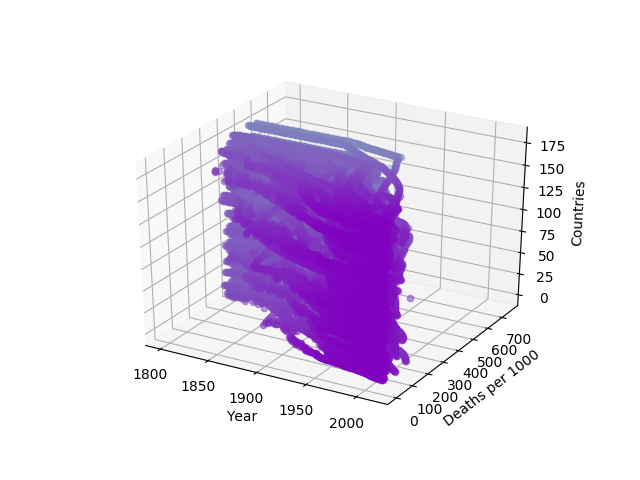
\includegraphics[width=\linewidth]{original1.png} \\
	\end{center}
		After parsing data into matrix from the given file, I've got:
		\begin{itemize}
		\item \(X = m \times n\) matrix, where \(m=180\) and \(n = 216\). 
		\item Number of features or dimensions \(d=216\). 
		\item Number of data-points  \(t=180\), where data-points are \(x^0....x^t\), each has dimension \(d\). \\
		\end{itemize}
	{\bf \item Part 1.} Principal Components Analysis (PCA). \\
	
	There are two ways to do dimensionality reduction in ML, feature selection and feature extraction. The PCA is the best known and the most widely used  feature extraction method.  As in all projection methods, in PCA we are interested in finding mapping from the original inputs in the original {\it d}-dimensional space to a new \((k < d)\)-dimensional space, with minimum loss of information. \\ 
	PCA  is an unsupervised method in that it does not use the output information and  the criterion that we want to maximize is the variance. 
	
	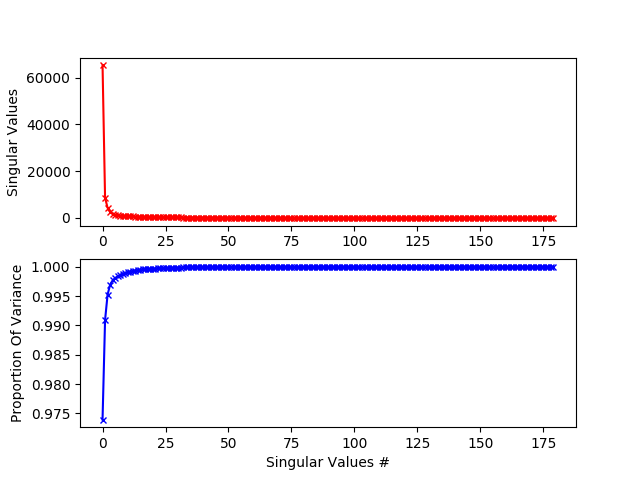
\includegraphics[width=\linewidth]{scree.png} \\
	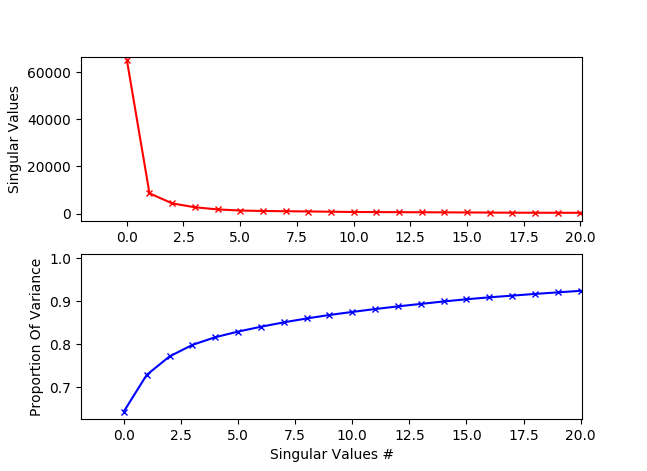
\includegraphics[width=\linewidth]{kpcs.png} \\
	\includegraphics[width=\linewidth]{ScatterPCs.png} \\
	{\bf \item Part 2.} K-mean clustering. \\
\end{enumerate}
	
\end{document} 